%! Suppress = MissingImport
\chapter{Related Work}\label{ch:background-literature}
There is a considerable amount of research in the area of pricing and resource allocation in cloud computing,
of which some use auction mechanisms to deal with competition~\citep{KUMAR2017234,Zhang2017,Du2019,Bi2019} as this
project does. Therefore section~\ref{sec:related-work-in-cloud-computing} presents the similar approaches to
resource allocation in cloud computing and edge cloud computing to the one taken in this project.

The proposed solution of the project (presented in chapter~\ref{ch:proposed-solution-to-problem}) uses a form of
machine learning, called reinforcement learning. Section~\ref{sec:related-work-in-machine-learning} explores the
research and the current state of the art algorithms of deep Q learning and policy gradient that are used in this
project.

\section{Related Work in Cloud Computing}\label{sec:related-work-in-cloud-computing}
A majority of approaches for pricing and resource allocation in cloud computing use a fixed resource allocation
mechanism such that user request a fixed amount of certain resource from the cloud provider. However this mechanism
provides no control over the resources quantity allocated to the server, only to which server these resources are
allocated to. Therefore a majority of this resources is focusing on designing efficient and incentive compatible
auction mechanism with~\cite{KUMAR2017234}, survey of these approaches.
% Todo on pricing on cloud computing
%~\citep{KUMAR2017234,Zhang2017,Du2019,Bi2019}.

Other closely related work on resource allocation in edge clouds~\cite{vaji_infocom} considers both the placement of
code/data needed to run a specific task, as well as the scheduling of tasks to different edge clouds. The goal there
is to maximize the expected rate of successfully accomplished tasks over time. Our work is different both in the setup
and the objective function. Our objective is to maximize the value over all tasks. In terms of the setup, they assume
that data/code can be shared and they do not consider the elasticity of resources.

Previous work by this author in~\cite{FlexibleResourceAllocation} proposed the novel resource allocation (explained in
chapter~\ref{ch:project-problem}) along with an optimisation problem mathematically describing the resource allocation.
The goal of the problem is to maximise the social welfare, the sum of all task values that are run and completed
successfully within the task deadline.
The paper presents three mechanism for the optimisation problem, one to maximise the social welfare and two auction
mechanisms. A greedy algorithm presented allows for quick approximation of a solution through the use of several
heuristics in order to maximise the social welfare. Results found that this mechanism could achieves over 90\% of the
optimal solution given certain heuristics compared to fixed resource allocatiom methods with only 70\% of
the solution solution. The algorithm is a polynomial time algorithm that will find solution within $\frac{1}{n}$
of the optimal social welfare. The heuristics were for ordering the task by density then for each task,
selecting a server based on available resource on each servers then to allocate resources that minimises the final
resource heuristics. The first of the auction mechanisms is a novel distributed iterative auction developed using
a reverse vcg principle~\citep{vickrey, Clarke, groves} to calculate a task price. That meant that a task doesnt need
to reveal its private value also that the auction could be run in a decentralised way. This means that the auction is
budget balanced however it is not economically efficient or incentive compatible. The mechanism achieves over 90\% of
the optimal solution due to its solving of the optimisation problem allowing it to find optimal resource allocations.
The third algorithm is an implementation of a single parameter auctions~\citep{nisan2007algorithmic_critical_value}
using the greedy algorithm (explained previously) to find the critical value of a task. Using this mechanism with
a monotonic value density heuristic results in the auction being incentive compatible also well a inherienting the
social welfare properties of the greedy mechanism.

\section{Related Work in Reinforcement learning}\label{sec:related-work-in-machine-learning}
Computer scientists have always been interested in testing computers against humans~\citep{turing_test} and a key
element of humans is the ability to learn from rewards. For computers this ability is much more complex and
researchers have found a variety of ways to allow computers to do this. These methods are broadly grouped into three
categories of supervised, unsupervised and reinforcement learning. Supervised learning uses pairs of inputs to true
outputs like in case of image classifications where each image has a correct category for the image to be mapped to.
Unsupervised learning instead doesn't have a true output meaning that algorithms tries to find links between similar data.

However both of these methods are not effective for real world interactions as agents must make a series of
actions that result in rewards. Algorithms designed for these problems with a series of actions fall into the category
of reinforcement learning which aims to maximise the agent rewards over time (an example environment has the
format~\ref{fig:reinforcement_learning}). This is the area of machine learning that this
project utilises as the problem can be modelled as a markov decision process (explained in section~\ref{sec:proposed-agents})
that allows agents to interact with the environment to learn over time. Reinforcement learning is a rapidly growing
field of research within AI due to its real world applications like driving a car, playing games, etc.

\begin{figure}
    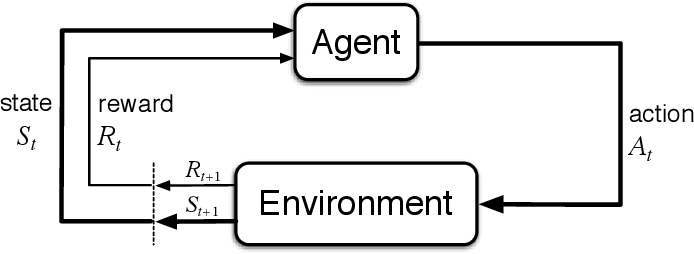
\includegraphics[width=10cm]{figures/reinforcement_learning.png}
    \caption{Reinforcement learning model (Source: ~\cite{Sutton1998})}
    \label{fig:reinforcement_learning}
\end{figure}

Q-learning algorithm~\cite{watkins1992q-learning} is a learning method used for estimating the action-value function,
one of the bases on for modern reinforcement learning. As the series of actions can be formed into a tree of
actions, an agent is interested in which actions will result in the largest reward in the future. This is formulated
as in equation~\eqref{eq:q_learning}.

\begin{align}
    Q(s_t, a_t) = E[R_{t+1} + \gamma R_{t+2} + \gamma^2 R_{t+2} + \cdots ] \label{eq:q_value} \\
    Q(s_t, a_t) = Q(s_t, a_t) + \alpha \cdot (r_t + \gamma \cdot \text{max}_a Q(s_{t+1} , a) - Q(s_t, a_t) ) \label{eq:q_learning} \\
\end{align}

However the curse of dimensionally was found to be a major problem as to use Q learning required
forming a table of state-actions in order to calculate and as the number of dimensions increase, the number of
state-actions will increase exponentially. Therefore making the method impractical for problem that had large state
space. Therefore use of a function approximate is used to circumvent this problem, traditionally done using a neural
network. Work by~\cite{atari} using a deep convolution neural network was able to achieve state of the art in six of seven
games tried on atari with three of these scores being superhuman. This work was followed up by~\cite{mnih2015humanlevel}
and found that with no modifications to the hyperparameters, neural network and training method; state of the art results were
achieved in almost all 49 atari games and superhuman results in 29 of these games. Additional heuristics have been
proposed for deep Q learning: double DQN~\citep{doubledqn}, prioritized experience replay~\citep{prioritizedexperiencereplay},
dueling network architecture~\citep{duelingdqn}, multi-step bootstrap targets~\citep{multi-step-dqn, Sutton1998},
A3C~\cite{A3C}, distributional Q-learning~\citep{distributional_dqn} and noisy DQN~\citep{noisy_dqn}. These methods were
combined to together~\cite{rainbow}, called rainbow DQN, achieving over 200\% of the original DQN algorithm and over
50\% than any optimisation on its own in a quarter of the observations.

Using the base of Q-learning, policy gradient~\ref{fig:actor-critic-model} separate the action selection policy to the
q-value policy. In Q-learning, the selection the action is based on the maximum Q-value of the actions however policy
gradient separates. This has the advantages of being able to deal with both discrete and continuous action spaces where
Q-learning can only deal with discrete action space. Also the learning method doesn't require $\epsilon$-greedy action
selection that can for Q-learning cause the resulting policy to differ from the optimal policy. Therefore policy
gradient has been used to master the game of Go~\citep{silver2017mastering} and achieve top 1\% in
Dota 2~\citep{OpenAI_dota} and Starcraft 2~\citep{starcraft2}.

\begin{figure}[h]
    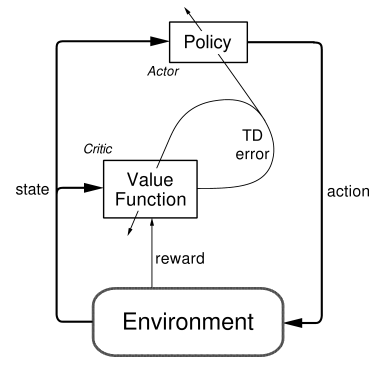
\includegraphics[width=10cm]{figures/actor-critic.png}
    \caption{Actor Critic model (Source: ~\cite{Sutton1998})}
    \label{fig:actor-critic-model}
\end{figure}